\documentclass[pdf]{prosper}

% Dualslide example for the `HA-Prosper' package.
% Created by: Hendri Adriaens
%             http://center.uvt.nl/phd_stud/adriaens
%             Center for Economic Research
%             Tilburg University, the Netherlands

%================================================
% Please also read the manual of HA-prosper and
% of the specific style you are using since some
% features of this example might not be supported
% by the style you use.
%================================================

\usepackage[toc,highlight,HA]{HA-prosper}

\title{Dualslide example for the HA-prosper package}
\subtitle{A package for use with prosper}
\author{Hendri Adriaens\\
\institution{CentER}\\
\institution{\href{http://center.uvt.nl/phd_stud/adriaens}{http://center.uvt.nl/phd\string_stud/adriaens}}}

\DefaultTransition{Wipe}
\TitleSlideNav{FullScreen}
\NormalSlideNav{ShowBookmarks}
\LeftFoot{\href{http://center.uvt.nl/phd_stud/adriaens}{Hendri Adriaens}, \today}
\RightFoot{Dualslide example for the HA-prosper package}

\begin{document}

% ==================================================================================
% Slide 1
\maketitle
% ==================================================================================


% ==================================================================================
% Slide 2
\overlays{5}{%
\begin{slide}{Dualslide 1}
\dualslide[linestyle=dashed,dash=4pt 4pt][linestyle=dotted]{%
lineheight=6cm,%
rfrheight=6cm,%
lfrheight=6cm,%
lcolwidth=.4\linewidth,%
rcolwidth=.54\linewidth}{%
  \begin{itemstep}
  \item HA-prosper also implements dualslides.
  \item This macro can be used to put content into two columns.
  \item One column can contain the text
  \hiddenitem
  \item and the other column for instance a figure.
  \end{itemstep}
}{%
  \fromSlide{4}{This is the figure:\par%
  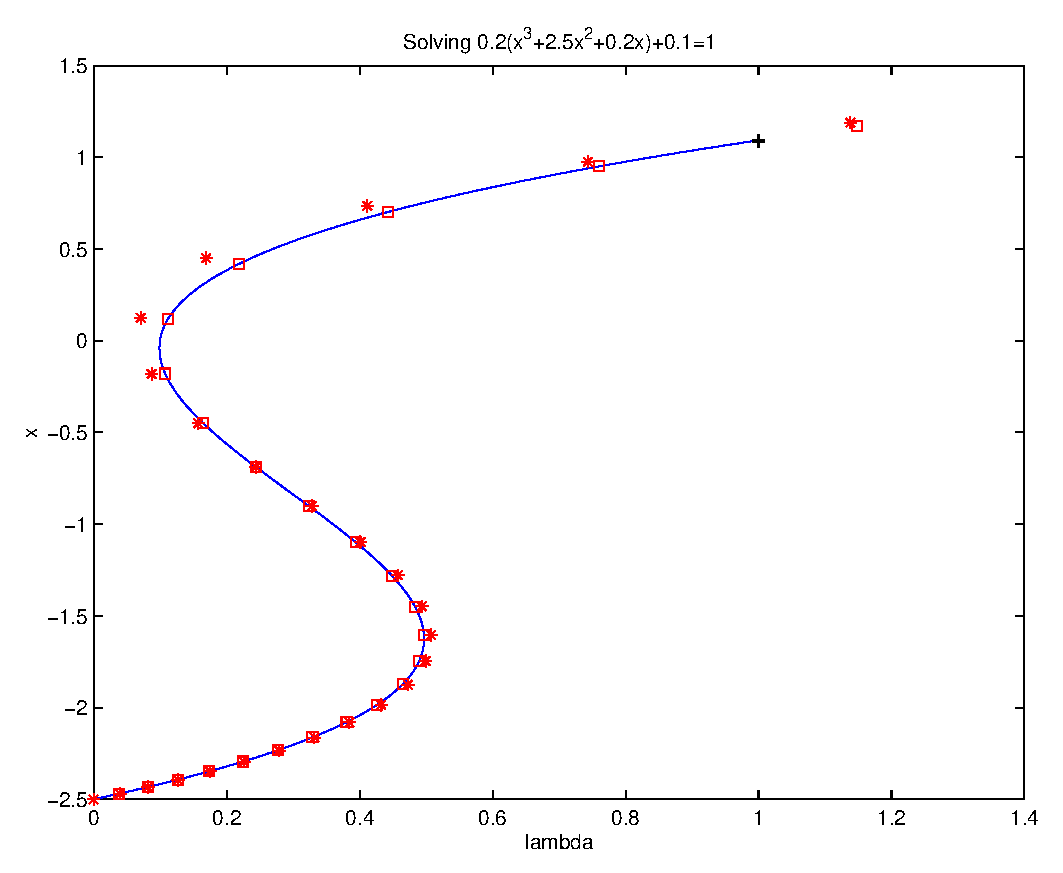
\includegraphics[scale=.3]{homotopy.eps}}%
}
\end{slide}
}
% ==================================================================================


% ==================================================================================
% Slide 3
\overlays{4}{
\begin{slide}{Dualslide 2}
\dualslide[shadow=true,shadowcolor=HAP@framecolor]{rfrheight=6cm}{%
  \begin{itemstep}
  \item You can also use the dualslide
  \item and the tools that prosper provides
  \end{itemstep}
}{%
  \begin{itemstep}[sstart=3]
  \item to continue a list
  \item in the right column.
  \end{itemstep}
}
\end{slide}
}
% ==================================================================================


% ==================================================================================
% Slide 4
\overlays{4}{
\begin{slide}{Dualslide 3}
This slide demonstrates top and bottom text and some prosper tools.
\dualslide{lineheight=4.2cm,topsep=.2cm}{
  \begin{itemstep}
  \item These are just some examples
  \item of the possibilities of prosper tools
  \item in combination with dualslide.
  \end{itemstep}
}{
  \onlySlide*{1}{\ding{110}\topbl{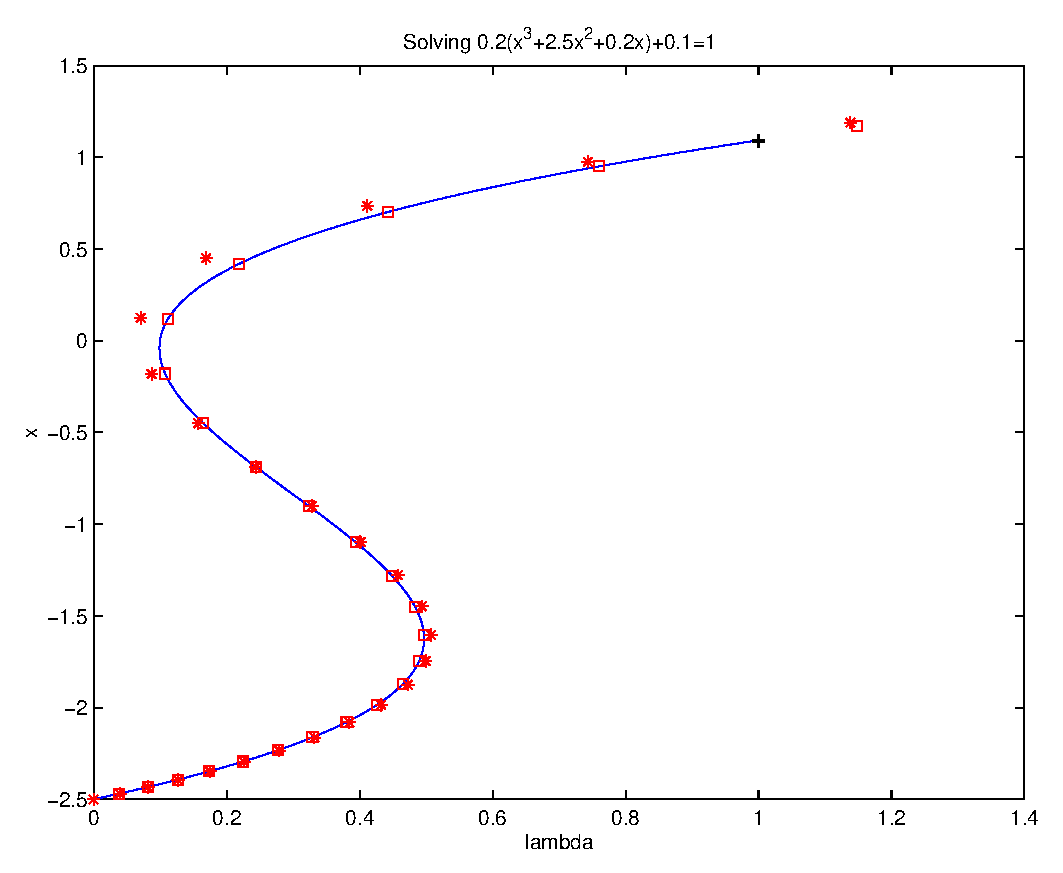
\includegraphics[scale=.1]{homotopy.eps}}\ding{110}}
  \onlySlide*{2}{\ding{110}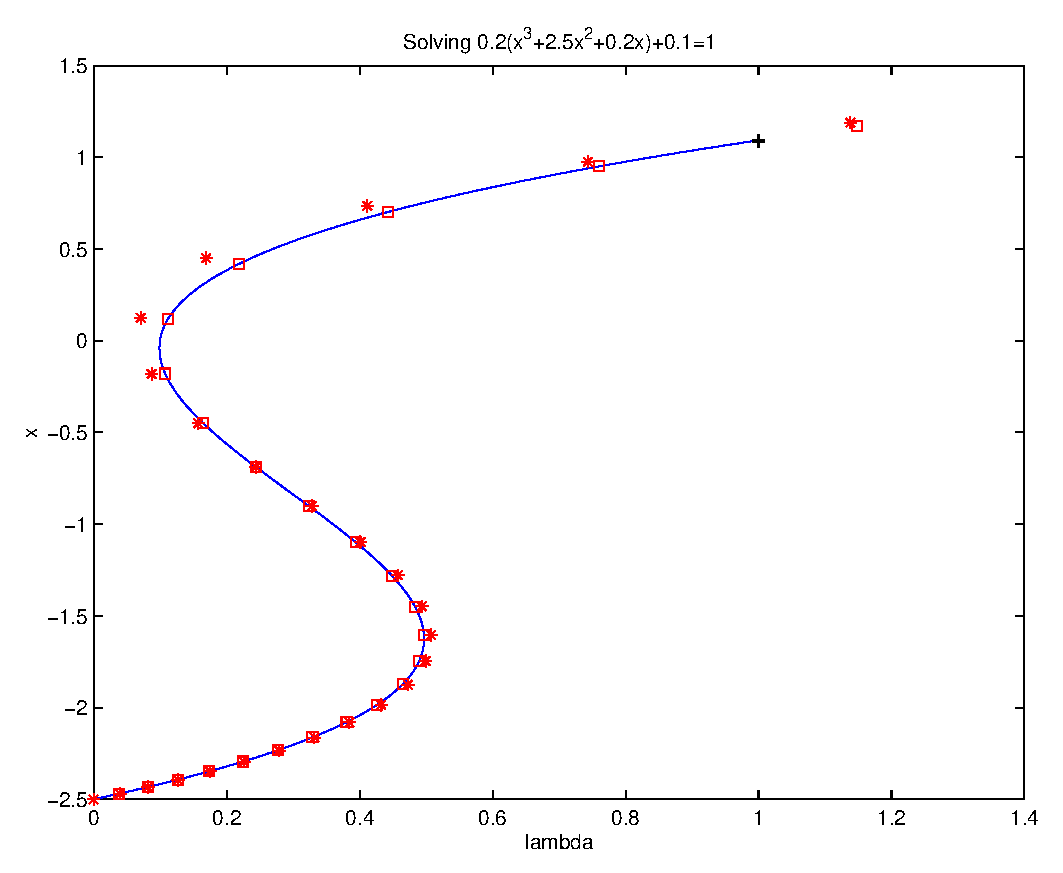
\includegraphics[scale=.1]{homotopy.eps}\ding{110}}
  \fromSlide{3}{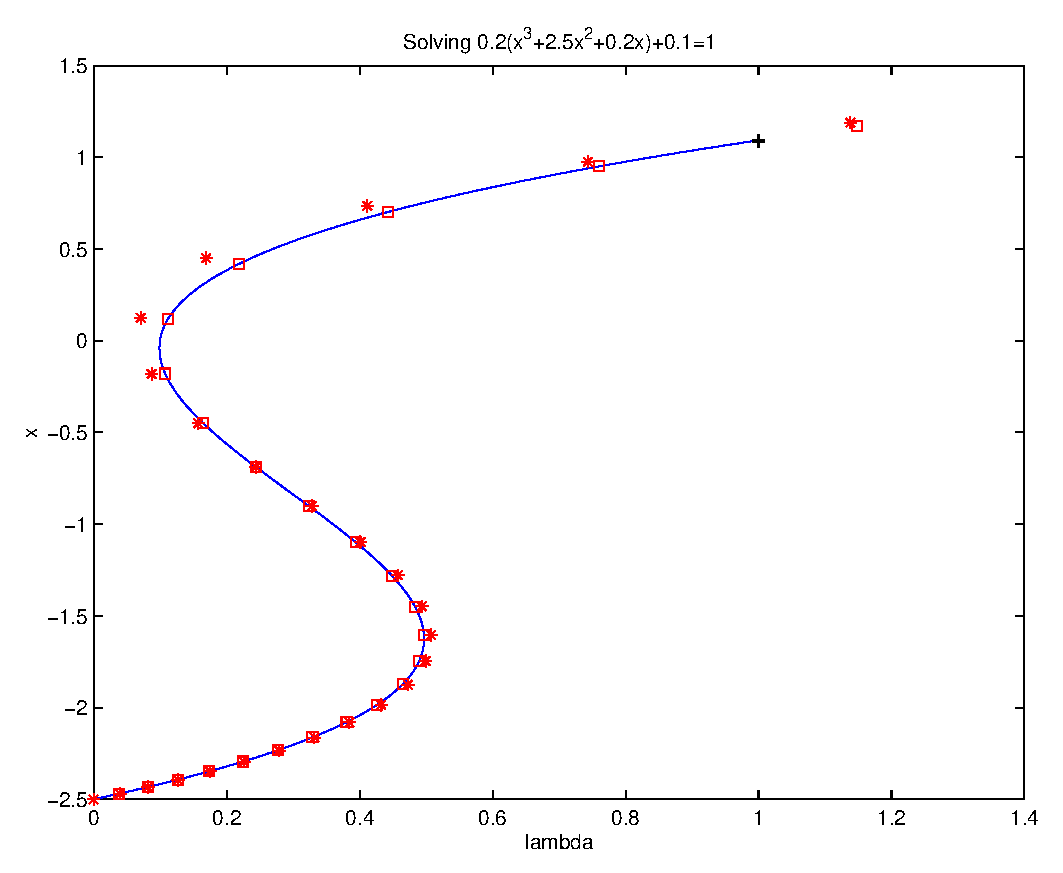
\includegraphics[scale=.2]{homotopy.eps}}
}
\fromSlide{4}{This is the end of the dualslide example.}
\end{slide}
}
% ==================================================================================


\end{document}
